
\section{Effective mass measurements}

\subsectoin{Temperature correction}

Effective mass measurements on particular extremal orbits rely on accurate temperature determination at all stages of the field sweep. On the Yellow magnet system, temperature from base of $\approx$\unit[0.3]{K} to $\approx$\unit[2]{K} is controlled by adjusting the He$^3$ sorbtion pump temperature and can be considered to be independant of field effect since the thermometer regulating the sorb temperature is outside of the strong field core. However if we consider \fig\ref{}, it is evident that there are magnetic field effects on the RuOx, which is mounted in the base of the magnet but thermally linked with the sample, and the Cernox thermometer that sits on the sample stage. Readings from both thermometers were taken with field sweeps from zero field up to \unit[18]{T} at steady temperatures \unit[0.30]{K}, \unit[0.53]{K}, \unit[0.64]{K}, \unit[1.06]{K} and \unit[1.34]{K}. By interpolating between this data\foonote{Performed using Python and Scipy's radial basis function class.}, reasonable corrections to some example thermometer readings can be achieved as is evident in the figure.

\subsubsection{Basic LK formula fitting}

A series of field sweeps were taken with $H$ at \unit[12]{\degree}, \unit[28]{\degree} and \unit[46]{\degree} from $[001]$ in the $[110]$ direction. These were performed at a variety of temperatures from base ($\approx\unit[0.3]{K}$) to above \unit[2]{K}. \Fig~\ref{Fig:3:ExampleLKFits} shows the Fourier amplitude of various peaks as a function of temperature along with fits to equation~\ref{Eqn:2:TempTermOscillationAmp}. The field range for the FFT was was necessarily large enough that individual peaks did not overlap and also could be observed across a reasonable range of temperatures but also small enough so that the $B$ dependent Dingle factor did not play too large a role and so an average $B$ field can be assumed. The results from these fits are shown in table \ref{Table:3:RetroFittedLKResults} along with the fit ranges. All FFTs in the plot were taken over an interval of \unit[12--18]{T} with the exception of the $\gamma_2$ fit which was taken between \unit[16-18]{T} so as to attain an appreciable peak. The standard deviationw as calculated by randomly varying the temperature values by the estimated error (\unit[0.06]{K}) 1000 times and then taking the standard deviation of the fitted $m^*$ values.
%%
\begin{figure}[h!]
    \begin{center}
        \includegraphics[scale=0.9]{Chapter3-dHvABaFe2P2/Figures/Mass/SimpleLKFits/SimpleLKFits}
        \caption{Fits to the temperature dependant part of the \LK formula. }
        \label{Fig:3:SimpleLKFits}
    \end{center}
\end{figure}
%%
Table \ref{Table:3:SimpleLKFitResults} also shows some results taken with a different field range. These fits give quite different values for the effective mass, indicating that the average field approximation is not a valid one.

\subsubsection{Retrofitting ansatz LK formulae}

The measurements presented in the previous section were further refined using the the ansatz LK formulae as described in section~\ref{Sec:2:LKRetrofitting}. \Fig~\ref{Fig:3:DingleTermExtractionFits} shows some sample fits used to extract the Dingle terms used in the ansatz fit functions.
%%
\begin{figure}[h!]
    \begin{center}
        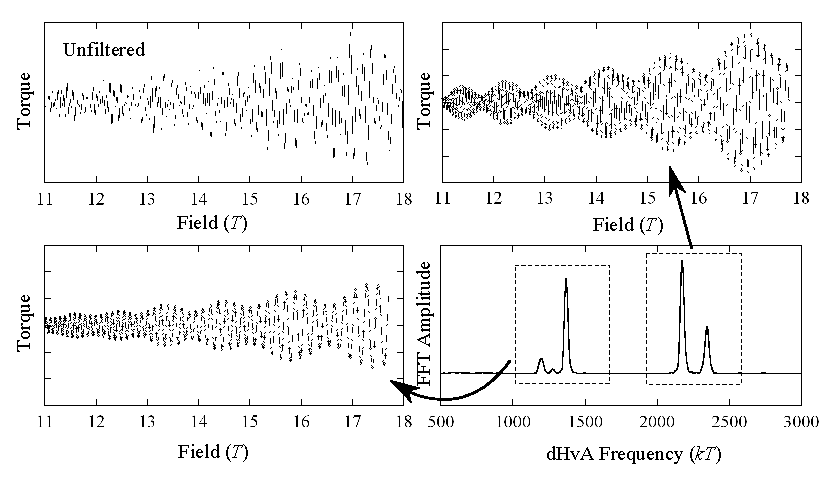
\includegraphics[scale=0.9]{Chapter3-dHvABaFe2P2/Figures/Mass/FittingDingleTerm/FittingDingleTerm}
        \caption{Top left panel shows torque data for data taken at \unit[12]{\degree} towards the $[110]$ direction at \unit[0.35]{K} with a polynomial background subtracted. Bottom right shows the FFT and the two filter windows to produce the filtered torque plots in the top right and bottom left. Filtered plots are fitted to extract the Dingle term for each frequency.}
        \label{Fig:3:DingleTermExtractionFits}
    \end{center}
\end{figure}
%%%%%
\begin{table}
    \begin{center}
        \caption{Details of the calculations for the retrofitted masses. $m^*$ values are given in terms of electron rest mass, $m_e$}
        \begin{tabular}[!h]{rrrrrrr}
\toprule
Angle	& Freq. (\unit[]{T})	& Label & $m^*$ & $m^*_{\textrm{retro}}$	& $\alpha$	& Field Lim. (\unit[]{T}) \\
\midrule
12	 & 1195	 & $\alpha_1$	 & 1.71(3)	& 1.75	& 58.681	& 12.0\\
12	 & 1195	 & $\alpha_1$	 & 1.49(2)	& 1.69	& 58.681	& 8.0\\
28	 & 1270	 & $\alpha_1$	 & 1.64(2)	& 1.68	& 59.602	& 12.0\\
46	 & 1540	 & $\alpha_1$	 & 1.86(3)	& 1.90	& 48.794	& 12.0\\
12	 & 1370	 & $\alpha_2$	 & 1.54(2)	& 1.58	& 45.989	& 12.0\\
28	 & 1526	 & $\alpha_2$	 & 1.69(2)	& 1.74	& 72.351	& 12.0\\
46	 & 2030	 & $\alpha_2$	 & 2.49(5)	& 2.56	& 61.058	& 12.0\\
28	 & 1370	 & $\alpha_3$	 & 1.85(3)	& 1.93	& 115.490	& 12.0\\
46	 & 1930	 & $\alpha_3$	 & 2.87(7)	& 3.04	& 149.390	& 12.0\\
12	 & 2176	 & $\beta_1$	 & 1.61(2)	& 1.65	& 51.119	& 12.0\\
12	 & 2353	 & $\beta_2$	 & 1.56(3)	& 1.62	& 102.360	& 12.0\\
12	 & 2353	 & $\beta_2$	 & 1.30(2)	& 1.87	& 102.360	& 6.0\\
28	 & 2603	 & $\beta_2$	 & 1.73(2)	& 1.76	& 34.082	& 12.0\\
46	 & 3335	 & $\beta_2$	 & 2.59(6)	& 2.69	& 94.572	& 12.0\\
28	 & 2472	 & $\beta_3$	 & 1.58(2)	& 1.61	& 48.807	& 12.0\\
46	 & 2972	 & $\beta_3$	 & 1.82(3)	& 1.86	& 40.033	& 12.0\\
46	 & 1320	 & $\gamma_1$	 & 2.13(5)	& 2.22	& 104.380	& 12.0\\
28	 & 920	 & $\gamma_1$	 & 2.19(3)	& 2.30	& 129.820	& 12.0\\
46	 & 4500	 & $\gamma_2$	 & 3.31(8)	& 3.32	& 91.057	& 16.0\\
12	 & 1285	 & $\delta_1$	 & 1.54(2)	& 1.64	& 173.000	& 12.0\\
28	 & 1370	 & $\delta_1$	 & 1.85(3)	& 1.93	& 115.490	& 12.0\\
46	 & 1630	 & $\delta_1$	 & 2.22(4)	& 2.33	& 126.020	& 12.0\\
\bottomrule
        \label{Table:3:RetroFittedLKResults}
        \end{tabular}
    \end{center}
\end{table}
%%
Table\ref{Tab:3:RetroFittedLKResults} lists the extracted Dingle terms for each peak of the Fermi surface and the subsequent results of the retrofitted calculations for the effective masses. The various field limits were chosen in order to either obtain a clearly delimited peak in the lower field cases or to obtain a signal from a weak peak in the higher field cases.


\subsubsection{`Microfitting' the LK formula}

A second attempt at refining the LK fits was performed by applying the microfit technique desribed in section~\ref{Sec:2:LKMicrofitting}. $1.5$ oscillations were fit at a time Filtering the data beforehand is not always straightforward due to close proximity of neighbouring peaks. The stronger peaks from the $\alpha$ and $\beta$ Fermi surfaces show banding of the masses and a clear trending of the results to one of a few values which have been highlighted in yellow. Data in these regions were averaged to give the values in table \ref{Table:3:MicroFitResults}.

All filtered using function $\textit{F}_{\textrm{filt}}(x) = \textit{F}(x) \times 1/2 [\tanh{(\pi(x - x_{\textrm{low}})/w)} + \tanh{(-\pi(x - x_{\textrm{high}})/w})]$ where $\textit{F}$ is the Fourier transform of the torque data, $x$ is the dHvA frequency, $x_{\textrm{low}}$ and $x_{\textrm{high}}$ are the lower and upper limits of the filter range respectively and $w$ determines the trail off slope of the filter function. For all measurements $w=10$.
%%
\begin{figure}[h!]
    \begin{center}
        \includegraphics[scale=0.7]{Chapter3-dHvABaFe2P2/Figures/Mass/MicroFits/MicroFits}
        \caption{Effective temperature dependant masses extracted from fits to between one and three dHvA oscillations in the measured data. See Appendix\ref{Appendix:MicroFitParams} for a full list of parameters for each set of fits.}
        \label{Fig:3:MicroFits}
    \end{center}
\end{figure}
%%
\begin{table}
    \begin{center}
        \caption{Details of the parameters used for the microfits. Effective masses given as a multiple of electron rest mass, $m_e$}
        \begin{tabular}[!h]{rrrrrrrr}
\toprule
Angle	& Freq. (\unit{T})	& Label	 & \multicolumn{2}{l}{Field (\unit[]{T})}  & \multicolumn{2}{l}{$m^*_{\textrm{microfit}}$}  & Filt. Width\\
        &                   &       & Max. & Min. & Mean & Stdev.   &   \\
\midrule
12	& 1210	& $\alpha_1$	& 17.0	& 11.0	& 1.75	& 0.03 &	1100--1240\\
28	& 1269	& $\alpha_1$	& 17.0	& 11.0	& 1.72	& 0.02 &	1200--1310\\
46	& 1532	& $\alpha_1$	& 17.0	& 9.0	& 1.92	& 0.02 &	1430--1585\\
12	& 1372	& $\alpha_2$	& 17.0	& 8.0	& 1.57	& 0.01 &	1320--1440\\
28	& 1530	& $\alpha_2$	& 17.0	& 8.0	& 1.75	& 0.02 &	1450--1650\\
46	& 2017	& $\alpha_2$	& 16.8	& 10.5	& 2.55	& 0.11 &	1970--2100\\
28	& 1365	& $\alpha_3$	& 17.0	& 9.5	& 1.97	& 0.03 &	1320--1440\\
46	& 1930	& $\alpha_3$	& 17.0	& 10.7	& 2.75	& 0.24 &	1890--1970\\
12	& 2180	& $\beta_1$	& 17.0	& 8.0	& 1.63	& 0.02 &	2100--2270\\
12	& 2350	& $\beta_2$	& 17.0	& 9.0	& 1.57	& 0.03 &	2270--2450\\
28	& 2605	& $\beta_2$	& 17.0	& 8.5	& 1.81	& 0.02 &	2555--2670\\
46	& 3347	& $\beta_2$	& 17.3	& 10.0	& 2.86	& 0.08 &	3250--3370\\
46	& 3381	& $\beta_2$	& 17.3	& 10.0	& 2.78	& 0.32 &	3365--2500\\
28	& 2475	& $\beta_3$	& 17.0	& 8.0	& 1.59	& 0.02 &	2400--2560\\
46	& 2970	& $\beta_3$	& 17.0	& 8.5	& 1.86	& 0.01 &	2850--3100\\
12	& 1270	& $\delta$	& 17.0	& 12.0	& 1.71	& 0.01 &	1250--1310\\
46	& 1626	& $\delta$	& 17.0	& 10.5	& 2.17	& 0.15 &	1590--1690\\
28	& 912	& $\gamma_1$	& 16.8	& 11.3	& 2.17	& 0.18 &	850--970  \\
46	& 1320	& $\gamma_1$	& 16.8	& 11.3	& 2.00	& 0.37 &	1270--1370\\
46	& 4497	& $\gamma_2$	& 16.8	& 12.2	& 3.31	& 0.13 &	4400--4600\\
\bottomrule
        \end{tabular}
        \label{Table:3:MicroFitResults}
    \end{center}
\end{table}

\begin{table}
    \begin{center}
        \caption{Summarised comparison of the three effective mass calculation techniques, further corrected by band mass, $m_b$, as found from DFT calculations.}
        \begin{tabular}[!h]{rrrrrrrr}
\toprule
Angle	& Freq. (\unit{T})	& Label	 & $m_b$	& $m^*/m_b$	& $m^*_{\textrm{retro}}/m_b$	& $m^*_{\textrm{microfit}}/m_b$ \\
\midrule
12	& 1210	& $\alpha_1$	& 1.04	& 1.64	& 1.68 & 1.68	\\
28	& 1269	& $\alpha_1$	& 0.90	& 1.83	& 1.88 & 1.92	\\
46	& 1532	& $\alpha_1$	& 1.00	& 1.86	& 1.90 & 1.92	\\
12	& 1372	& $\alpha_2$	& 0.84	& 1.83	& 1.88 & 1.86	\\
28	& 1530	& $\alpha_2$	& 0.93	& 1.81	& 1.87 & 1.88	\\
46	& 2017	& $\alpha_2$	& 1.83	& 1.36	& 1.40 & 1.40	\\
28	& 1365	& $\alpha_3$	& 1.18	& 1.56	& 1.63 & 1.67	\\
46	& 1930	& $\alpha_3$	& 1.00	& 2.87	& 3.04 & 2.75	\\
12	& 2180	& $\beta_1$ 	& 0.98	& 1.64	& 1.68 & 1.66	\\
12	& 2350	& $\beta_2$ 	& 0.86	& 1.81	& 1.88 & 1.82	\\
28	& 2605	& $\beta_2$ 	& 1.03	& 1.68	& 1.71 & 1.76	\\
46	& 3347	& $\beta_2$ 	& 1.80	& 1.44	& 1.50 & 1.59	\\
46	& 3381	& $\beta_2$ 	& 1.80	& 0.88	& 0.90 & 1.55	\\
28	& 2475	& $\beta_3$ 	& 0.93	& 1.95	& 2.00 & 1.71	\\
46	& 2970	& $\beta_3$ 	& 1.03	& 2.07	& 2.15 & 1.80	\\
12	& 1270	& $\delta$  	& -0.91	& -2.41	& -2.53& -1.88	 \\
46	& 1626	& $\delta$  	& -1.10	& -3.00	& -3.01& -1.96	 \\
28	& 912	& $\gamma_1$	& -1.49	& -1.03	& -1.10& -1.46	 \\
46	& 1320	& $\gamma_1$	& -2.04	& -0.91	& -0.95& -0.98	 \\
46	& 4497	& $\gamma_2$	& -1.89	& -1.17	& -1.23& -1.75	 \\
\bottomrule
        \end{tabular}
        \label{Table:3:EffectiveMassResults}
    \end{center}
\end{table}
